\documentclass[12pt,french]{article}

	\usepackage{babel}
	\usepackage[autolanguage]{numprint}
	\usepackage[utf8]{inputenc}
	\usepackage[T1]{fontenc}
	
	%Pour paragraphe
	\usepackage{parskip}
	
	
	%Utile pour page titre
	\usepackage[charter]{mathdesign}
	\usepackage{graphicx} 
	\usepackage[a4paper,bindingoffset=0.2in,left=1in,right=1in,top=1in,bottom=1in]{geometry}
	
	%Pour image
	\usepackage{graphicx}
	\graphicspath{ {./images/} } %path image
	
	% Pour math
	\usepackage{amsmath}
	
	\usepackage{bm} %pour gras \bm{character}
%---------------------------------------
	


\begin{document}


%L'étoile permet de pas afficher le 1 devant
\section*{Pipeline}
\subsection*{Explication rapide}
En gros le but de la pipeline c'est de prendre un data set pandas, de lui appliquer des transformations (ex: transformer notre query en vecteur numérique). Une fois les transformations appliquées, on peu utiliser un classificateur pour faire nos prédictions. 

On peu utiliser un grid search sur toute notre pipeline, autant pour optimiser nos transformations que les paramètres de notre classificateur.

Les méthodes score, predict, fit, etc fonctionne sur une pipeline.

On peut assembler des pipeline l'une à la suite de l'autre.

\subsection*{Pipeline dans notre code à nous}
Les trucs importants se passent dans basis\_pipeline.py. Notre pipeline est séparée en 2 partie, la partie \emph{Transformer} et la partie \emph{Classifier}. 

Voici la pipeline de trnasformation :

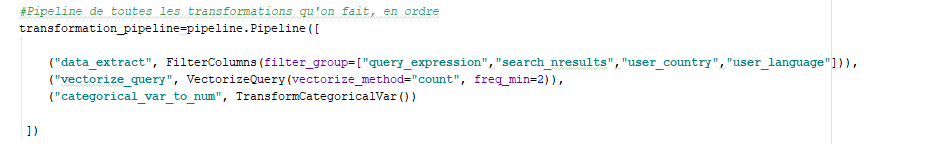
\includegraphics[width=\linewidth]{trans_pipe}

Chacune des 3 lignes représente une transformation qu'on fait sur notre data frame. par exempel vectorize\_query prend la query, la transform en vecteur numérique et retire la query textuelle du data frame. Toutes ces transformations se font une après l'autre. On peut ajouter d'autre \emph{transformer} éventuellement.


\section*{Grid search avec pipeline}

Pour tester toutes les combinaisons possibles, on se définit une grille de paramètres à explorer:

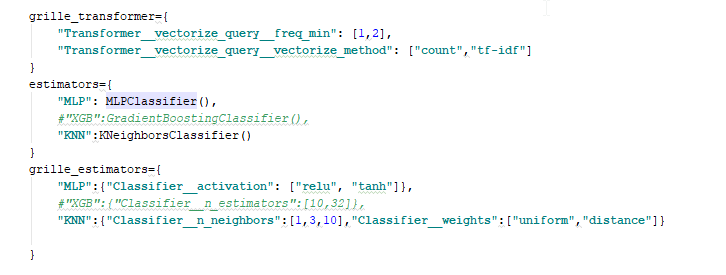
\includegraphics[width=\linewidth]{grid}

Une grille pour les paramètres de notre pipeline de transformation, un dict avec nos modèles et un dict avec nos paramètres de classificateur à tester. Il faut respecter la structure si on veut en ajouter d'autre. Les classificateurs doivent avoir la méthodes .predict\_proba() pour pouvoir être utilisés, car on fait le grid search avec le score de coveo

J'ai créé de quoi qui permet de tester tout ça:

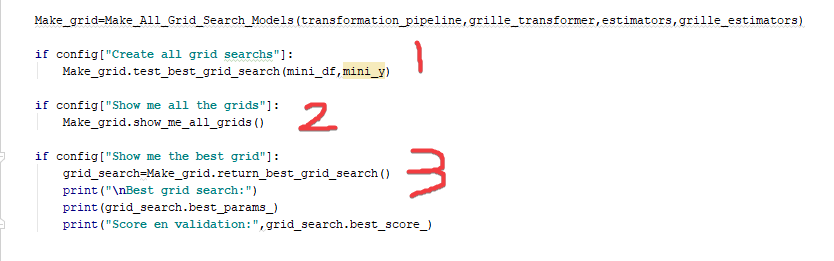
\includegraphics[width=\linewidth]{etapes_grid}

1. ça permet de créer un fichier avec pickle qui sauvergarde une liste qui contient un objet grid search pour chacun des classificateur qu'on utilise (le fichier est list\_grid\_search.p).

2. permet de print toutes les combinaisons testées 

3. retourne le meilleur objet grid search qu'on peut ensuite utiliser

\section*{Améliorations}
Pour l'instant on utilise seulement une partie de nos données, on prend juste les search qui résulte en un click, puis ceux sans click ne sont pas utilisés (donc 52 000-25 000 ish données sont tout simplement pas utilisées).

Je suis pas mal sûr que y'a de quoi à faire avec ces données là. En leur attribuant par exemple un document en regardant les visits antérieurs de l'utilisateur avec le visit id et le click date time.  Ex : si un gars cherche "I want to know what is the best restaurant to eat on my first date with this awesome chikita I met on Tinder" et ne click sur rien, puis 2 minutes après il cherche : "good restaurant" et il clique sur de quoi, on peut assumer qu'on aurait pu lui renvoyer ce document trouvé dès sa première querry trop longue.

Je propose qu'une petite équipe travaille sur ça, car je pense qu'on peut vraiment aller chercher de quoi. C'est également simple de travailler de façon indépendante sur ça, pendant qu'une autre équipe travaille sur autre chose. J'ai commencer à faire un frame de fonction dans le fichier import\_data.py :

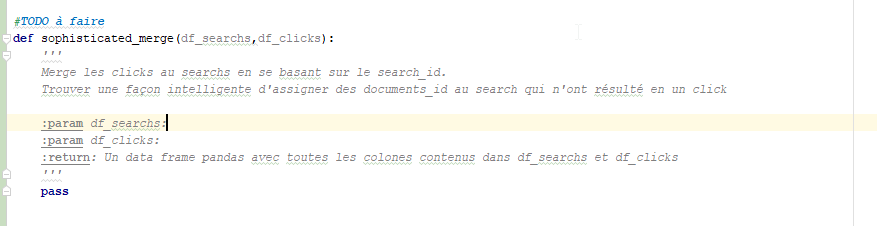
\includegraphics[width=\linewidth]{awesome_merge}

Il resterait à la compléter. C'est quand même une grosse job à faire !

\end{document}
